\section{Approximating Elasticity Tensors}
\label{sec:62tensors}

\paragraph{Optimization process}

\minitoc{75mm}{7}

During the process of solving \cref{eq:topoOptProblemDiscrete},
optimization algorithms typically
evaluate the objective function $\compliance(\mcp{1}, \dotsc, \mcp{M})$
iteratively at different \term{micro-cell parameter combinations}
$(\mcp{1}, \dotsc, \mcp{M}) \in (\real^d)^M$.
Every evaluation of $\compliance$ corresponds to one solution of a
macro-problem.
However, to solve the macro-problem,
the elasticity tensors $\etensor^{(q)}$ of all $M$ macro-cells
need to be known.
Hence, in every optimization iteration, it is necessary to solve
one macro-problem and $M$ micro-cell problems,
all with the \fem.
This naive approach has two major drawbacks, which we explain in
the following.



\subsection{Drawbacks of the Naive Approach}
\label{sec:621drawbacks}

\paragraph{Drawback 1: Computation time}

First, this approach is computationally infeasible
even for simple micro-cell models and optimization scenarios.
The computation of a single elasticity tensor usually takes seconds to
minutes.
All $M$ micro-cell problems per optimization iteration
can be solved in parallel without any communication.
However, $M$ is typically in the range of thousands and
there are thousands or tens of thousands optimization iterations
(the optimization problem is $(d \cdot M)$-dimensional!).
This implies that the overall computation may still take
several days or even weeks to complete.

\paragraph{Drawback 2: Approximation of gradients}

Second, most optimization algorithms require gradients of the
objective function and of the constraints, i.e.,%
\begin{equation}
  \partialderiv{\partialdiff{} x_t}{\etensor^{(q)}}(\mcp{q}),\quad
  \partialderiv{\partialdiff{} x_t}{\denscell^{(q)}}(\mcp{q}),\qquad
  q = 1, \dotsc, M,\quad
  t = 1, \dotsc, d.
\end{equation}
However, in general, both gradients are unavailable and
have to be approximated by finite differences.
This introduces new error sources and
increases the number of elasticity tensors to be evaluated,
further slowing down the solution process.
Additionally, the number of optimization iterations necessary to
achieve convergence might increase
if there are discontinuities in the objective function
or its gradient.
Such discontinuities can already be caused by the inexact solution of the \fem.
If we need Hessians or other higher-order derivatives,
then the issues even worsen.



\subsection{B-Splines on Sparse Grids for Topology Optimization}
\label{sec:622BSplines}

\paragraph{Elasticity tensor function}

As a remedy, we replace the costly elasticity tensors with cheap surrogates.
If we assume that all macro-cells use the same micro-cell model,
the elasticity tensor $\etensor^{(q)}$ of the $q$-th macro-cell
with the parameter $\mcp{q} \in \clint{\*0, \*1}$
can be written as the value $\etensor(\mcp{q})$ of some function
$\etensor\colon \clint{\*0, \*1} \to \real^{6 \times 6}$
(assuming that $\dimobjdomain = 3$) at the point $\mcp{q}$.
In the following,
$\etensor\colon \clint{\*0, \*1} \to \real^m$
gives $m \in \nat$ values from which the symmetric elasticity tensor
can be uniquely reconstructed,
i.e., $m = 6$ for $\dimobjdomain = 2$ and $m = 21$ for $\dimobjdomain = 3$.
The vector-valued/matrix-valued versions of $\etensor$
will be used interchangeably.

\paragraph{Elasticity tensor surrogate}

The idea is to use B-splines on sparse grids to approximate
the elasticity tensor function $\etensor$.
In contrast to the theoretical framework that we established in
\cref{chap:20sparseGrids,chap:30BSplines,chap:40algorithms},
the function to be interpolated is not scalar-valued, but vector-valued.
This means that we have to construct $m$ sparse grid interpolants
$\etensorentryintp{j}$
for the $m$ components $\etensorentry{j}$ of $\etensor$ ($j = 1, \dotsc, m$).
Note that one could generate different spatially adaptive sparse grids for the
different components $\etensorentryintp{j}$.
However, it is not possible to evaluate only specific entries of $\etensor$
without also evaluating all other entries,
which means that we would waste computational resources by selecting only
a subset of the calculated entries.
Therefore, we use the same grid for all components.

Additionally, we approximate the density $\denscell^{(q)}$
of the $q$-th macro-cell with a surrogate $\denscellintp$ using
B-splines on the same sparse grid as for $\etensorentryintp{j}$
for reasons of implementation,
resulting in $m + 1$ sparse grid interpolants in total.
From a theoretical perspective, this is not necessary,
since the density can be explicitly calculated with simple formulas
for most micro-cell models, independently of evaluations of the
elasticity tensor.

\paragraph{Advantages}

Our approach has multiple obvious advantages:
\begin{itemize}
  \item
  The sparse grid interpolant $\etensorintp$ has to be generated only
  once in an \term{offline step} before the optimization algorithm starts.
  During the optimization \term{(online phase),}
  only inexpensive evaluations of $\etensorintp$ are performed,
  saving much computation time.
  
  \item
  Sparse grids ease the curse of dimensionality, which prohibits
  conventional full grid interpolation methods if $d > 4$.
  
  \item
  With spatially adaptive sparse grids and a suitable refinement criterion,
  we can spend more grid points in regions of interest of $\etensor$,
  e.g., regions with large oscillations.
  
  \item
  By using B-splines as basis functions,
  the interpolant $\etensorintp$ will be more accurate
  than with piecewise linear basis functions.
  In addition, we can calculate its derivatives
  $\tpartialderiv{\partialdiff{} x_t}{\etensorintp}(\mcp{q})$
  fast and explicitly,
  accelerating the speed of convergence of the optimizer.
\end{itemize}



\breakpagebeforenextheadingtrue
\subsection{Cholesky Factor Interpolation}
\label{sec:623cholesky}

\paragraph{Positive definiteness of elasticity tensors}

Unfortunately, just replacing elasticity tensors with
B-spline surrogates often does not lead to correct results in practice.
Experiments show that for only for some sparse grids,
the optimization algorithm converges to an optimal point
\cite{Valentin16Hierarchical}.
The optimization algorithm crashes for most spatially adaptive grids,
not being able to find any meaningful optimum.
%
The root of the problem proves to be that
the interpolated elasticity tensors $\etensorintp(\*x)$ are not
positive definite for specific
micro-cell parameters $\*x \in \clint{\*0, \*1}$.
However, indefinite or even negative definite tensors $\etensorintp$
would mimic unphysical behavior.%
\footnote{%
  In the scalar case, this is analogous to Hooke's law for linear springs,
  where the force $F = kx$ needed to displace the end of a spring
  (fixed at the other end) by $x$ is proportional to $x$.
  The proportionality constant $k$ (which corresponds to the elasticity tensor)
  has to be positive.%
}
Hence, it is imperative for the optimization process that
the interpolated elasticity tensors are \spd.

\paragraph{Positive definiteness of sparse grid interpolants}

Interpolation on sparse grids per se does not preserve
positive definiteness.
A counterexample is shown in \cref{fig:cholesky1},
which displays the minimal eigenvalue of the elasticity tensor surrogate
resulting from interpolation on a regular sparse grid.
As the positivity of the diagonal is a necessary condition
for positive definiteness,
small oscillations of the interpolant of some entries
already make the whole elasticity tensor non-positive-definite.

\begin{figure}
  \subcaptionbox{%
    Minimal eigenvalue of $\etensorintp(\*x)$%
    \label{fig:cholesky1}%
  }[65mm]{%
    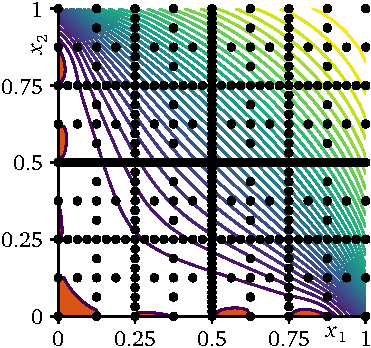
\includegraphics{cholesky_1}%
  }%
  \hfill%
  \subcaptionbox{%
    Minimal eigenvalue of $\etensorcholintp(\*x)$%
    \label{fig:cholesky2}%
  }[65mm]{%
    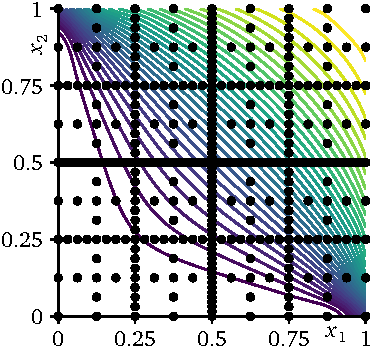
\includegraphics{cholesky_2}%
  }%
  \hfill\hfill%
  \raisebox{2.2mm}{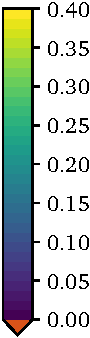
\includegraphics{cholesky_3}}%
  \caption[%
    Minimal eigenvalue of interpolated elasticity tensors%
  ]{%
    Minimal eigenvalue \emph{(colored contour lines)}
    of elasticity tensor surrogates
    for the 2D cross model ($\dimobjdomain = 2$, $d = 2$)
    \vspace{-0.3em}%
    and cubic hierarchical B-splines $\bspl{\*l,\*i}{p}$ ($p = 3$) on
    the regular sparse grid $\coarseregsgset{n}{d}{b}$ \emph{(dots)}
    with $n = 6$ and $b = 4$.
    \emph{Left:} The minimal eigenvalue of $\etensorintp(\*x)$
    becomes negative in some regions \emph{\textcolor{C1}{(red areas)}}
    of the domain $\clint{\*0, \*1}$,
    indicating that $\etensorintp(\*x)$ is not positive definite.
    \emph{Right:} The minimal eigenvalue of $\etensorcholintp(\*x)$
    is non-negative in the whole domain $\clint{\*0, \*1}$.%
  }%
  \label{fig:cholesky}%
\end{figure}

These oscillations are more likely to occur near the boundary of the domain
$\clint{\*0, \*1}$, such that there are larger regions
where the interpolated tensor is not positive definite anymore.
The reason is two-fold:
First, sparse grids without boundary points
are notoriously biased towards the center of the domain,
as they place only few points near the boundary \cite{Pflueger10Spatially}.
This leads to a loss of interpolation accuracy near the boundary
when compared to the center of $\clint{\*0, \*1}$.
Second, both the minimal eigenvalue of $\etensor(\*x)$ and the norm of its
gradient with respect to $\*x$ are small near $x_1 = 0$ or $x_2 = 0$.
Consequently, the ``surface'' of the minimal eigenvalue function
is rather flat in these regions and almost vanishes,
facilitating the existence of negative eigenvalues of
surrogate functions $\etensorintp(\*x)$.

Note that for most micro-cell models,
the optimization algorithm often evaluates the objective function
$\compliance(\mcp{1}, \dotsc, \mcp{M})$ at micro-cell parameter
combinations for which many of the points $\mcp{j}$ are near the boundary
of $\clint{\*0, \*1}$.
This is because many of the macro-cells will either be empty or
fully filled with material, which usually corresponds to micro-cell
parameters near zero or one, respectively.
Thus, $\etensorintp$ is frequently evaluated in the regions of
indefiniteness, which further worsens the issue.

\pagebreak

\paragraph{Positivity-preserving methods}

Even in one dimension, it cannot be guaranteed that the interpolant of
positive data remains positive,
which is a key problem in the estimation of probability densities
\multicite{Pflueger10Spatially,Griebel10Finite,Franzelin16From}.
Just clamping the interpolated values via $\max(\cdot, 0)$ does not help:
In our application, the tensor may still be indefinite;
additionally, the calculated gradients of the interpolants do not match
the actual gradients anymore.
In density estimation, clamping a density-like function changes its
integral, making it necessary to recalculate its normalization constant
\cite{Franzelin17Data}.

One possible workaround is to apply a continuous injective transformation
$T\colon \posreal \to \real$ on the positive values (e.g., $\ln$),
then interpolate the resulting values, and finally
apply the inverse transformation $T^{-1}\colon \real \to \posreal$
on the interpolated values (e.g., $\exp$).%
\footnote{%
  Formally, the inverse function $T^{-1}\colon T(\posreal) \to \posreal$
  is only defined on the image $T(\posreal)$ of $T$,
  which might not be the whole real line.
  However, we assume that $T^{-1}$ can be ``reasonably'' extended to $\real$
  (e.g., $T \ceq \sqrt{\cdot}$ and $T^{-1} = ({\cdot})^2$).%
}
For the piecewise linear hierarchical basis, another approach has been
developed recently \cite{Franzelin17Data},
maintaining the positivity by inserting additional sparse grid points.
In the context of spline approximation,
positivity-preserving approximation schemes based on so-called
quasi-interpolation are known \cite{Hoellig13Approximation}.
For our application, for which we need to preserve positive definiteness,
it is conceivable that one could apply these positivity-preserving
methods in the eigenspace,
interpolating the positive eigenvalues.

\paragraph{Interpolation of Cholesky factors}

Instead, we pursue a different, more canonical
approach based on Cholesky factorization:

\begin{proposition}[Cholesky factorization]
  For every \spd matrix $\etensor \in \real^{6 \times 6}$,
  there is a unique upper triangular matrix
  $\cholfactor \in \real^{6 \times 6}$
  with positive diagonal entries such that
  \begin{equation}
    \etensor
    = \tr{\cholfactor} \cholfactor.
  \end{equation}
\end{proposition}

\begin{proof}
  See \cite{Benoit24Note} or \cite{Freund07Stoer}.
\end{proof}

In one dimension, the Cholesky factorization is equivalent
to the application of a transformation $T$ as above by choosing
$T \ceq \sqrt{\cdot}$ and $T^{-1} = (\cdot)^2$.
Our approach is as follows:
\begin{enumerate}
  \item
  Define $\cholfactor\colon \clint{\*0, \*1} \to \real^{6 \times 6}$
  as the Cholesky factor of
  $\etensor\colon \clint{\*0, \*1} \to \real^{6 \times 6}$, i.e.,
  $\etensor(\*x) = \tr{\cholfactor(\*x)} \cholfactor(\*x)$
  for all $\*x \in \clint{\*0, \*1}$.
  
  \item
  During the grid generation (offline phase),
  evaluate $\etensor(\gp{\*l,\*i})$ at the grid points $\gp{\*l,\*i}$,
  compute the Cholesky factors $\cholfactor(\gp{\*l,\*i})$ of
  $\etensor(\gp{\*l,\*i})$,
  and interpolate them instead of the elasticity tensors
  to obtain an interpolant
  $\cholfactorintp\colon \clint{\*0, \*1} \to \real^{6 \times 6}$.
  
  \item
  During the optimization (online phase),
  every time the value $\etensor(\*x)$ of an elasticity tensor is needed,
  the interpolant $\cholfactorintp(\*x)$ is evaluated and we return
  \begin{equation}
    \etensorcholintp(\*x)
    \ceq \tr{\cholfactorintp(\*x)} \cholfactorintp(\*x).
  \end{equation}
\end{enumerate}

\paragraph{Advantages of Cholesky factor interpolation}

As shown in \cref{fig:cholesky2},
the resulting elasticity tensor surrogate $\etensorcholintp$
is positive semidefinite on the whole domain and
positive definite almost everywhere:
The surrogate $\etensorcholintp(\*x)$ is singular if and only if
$\cholfactorintp(\*x)$ is singular, which is in general
only the case on a negligible null set in $\clint{\*0, \*1}$.

Another advantage of this approach is that not only the
positive definiteness, but also the explicit differentiability
of the surrogate $\etensorcholintp$ is preserved.
The gradient can be computed easily and fast with the product rule:
\begin{equation}
  \label{eq:choleskyFactorDerivative}
  \partialderiv{\partialdiff{} x_t}{\etensorcholintp}(\*x)
  = \tr{\cholfactorintp(\*x)} \cdot
  \partialderiv{\partialdiff{} x_t}{\cholfactorintp}(\*x) +
  \tr{\partialderiv{\partialdiff{} x_t}{\cholfactorintp}(\*x)} \cdot
  \cholfactorintp(\*x),\quad
  t = 1, \dotsc, d,
\end{equation}
where both the sparse grid interpolant $\cholfactorintp(\*x)$ and
its derivative $\partialderiv{\partialdiff{} x_t}{\cholfactorintp}(\*x)$
are known.
As discussed above,
this is key to the applicability of gradient-based optimization.
